\documentclass{article}

\usepackage{xeCJK}
\setCJKmainfont{SimSun}

\title{FPGA Homework IV}
\author{李约瀚 \\ 14130140331 \\ qinka@live.com \\ me@qinka.pro \\ qinka@qinka.pw(remove soon)}

\usepackage{listings}
\usepackage{hyperref}

\begin{document}
    \maketitle
    \newpage
    \tableofcontents
    \newpage
    \section{Summary}
    \label{sec:summary}
    
    In this homework, I try to describe a one-bit comparator in VHDL.
    I use both of \lstinline[language=VHDL]|xor| and with-select notation to represent a comparator. 
    The delay of the one with with-select notation is short than ones which is using \lstinline[language=VHDL]|xor|.
    When the frequency of the input signals  are higher then 50MHz,
    the delay of the one, which is using \lstinline[language=VHDL]|xor|, can not be ignored,
    and it has effects on other signals. However, The one with with-select notation is well.

    There are also the behaviorl simulation and the post-route simulation of the comparator.
    And there is also RTL schematics.


    \section{Represent}
    \label{sec:represent}

    For such a comparator, it will return a ``true'' signal, in logic, when the two input signals are same, in logic.
    So it is smae with ``xor''. Then the first idear of the comparator is using ``xor''. And then we can also use with-select notation.
    And the following codes is the sources of comparator.

    Firstly, we need using the libraries from IEEE.

\begin{lstlisting}[language=VHDL]
library IEEE;
use IEEE.STD_LOGIC_1164.ALL;
\end{lstlisting}

    Then I need to define the comparator.

\begin{lstlisting}[language=VHDL]
entity comparator is
  port( A : in  STD_LOGIC
      ; B : in  STD_LOGIC
      ; C : out STD_LOGIC
      );
ebd comparator;
\end{lstlisting}

    Then I represent the comparator with ``xor''.

\begin{lstlisting}[language=VHDL]
architecture xor_one of comparator is
begin
  C <= A xor B;
end xor_one;
\end{lstlisting}
    
    Then it is the one using with-select notation.

\begin{lstlisting}[language=VHDL]
architecture with_one of comparator is
  signal I : STD_LOGIC_VECTOR(1 downto 0);
begin
  with I select
  C <= '1' when '11',
       '1' when '00',
       '0' when others;
  I(0) <= A;
  I(1) <= B;
end with_one;
\end{lstlisting}



    \section{Test Bench}
    \label{sec:testbench}

    Here I need to simulate the two of the comparator, so I write one test bench with the both of the kinds of comparator.

\begin{lstlisting}[language=VHDL]
library IEEE;
use IEEE.STD_LOGIC_1164.ALL;
 
ENTITY tb_comparator IS
END tb_comparator;
\end{lstlisting}

    \textit{in this ``architecture''}
\begin{lstlisting}[language=VHDL]
ARCHITECTURE behavior OF tb_comparator IS 
\end{lstlisting}
    
    To test this comparator, firstly, we need to write down the component declaration for the unit under test.

\begin{lstlisting}[language=VHDL]
  component comparator
  port( A :  IN std_logic
      ; B :  IN std_logic
      ; C : OUT std_logic
      );
  END COMPONENT;
\end{lstlisting}

    The I define the signals used in this architecture. 

\begin{lstlisting}[language=VHDL]
  signal A : std_logic := '0';
  signal B : std_logic := '0';
  signal C : std_logic_vector(1 downto 0) := "00";
\end{lstlisting}

    Also, I define the period of the clock which control the input signals' frequency.

\begin{lstlisting}[language=VHDL]
  constant clock_period : time := 20 ns;
\end{lstlisting}

   Instantiate the unit under test.

\begin{lstlisting}[language=VHDL]
BEGIN
  uut_xor: comparator PORT MAP (
          A => A,
          B => B,
          C => C(0)
        );
  uut_with: comparator PORT MAP (
          A => A,
          B => B,
          C => C(1)
        );
\end{lstlisting}

   The main process for the simulation is the following.

\begin{lstlisting}[language=VHDL]
  stim_proc: process
  begin		
	A <= '0';
	B <= '0';
	wait for clock_period;
	A <= '0';
	B <= '1';
	wait for clock_period;
	A <= '1';
	B <= '0';
	wait for clock_period;
	A <= '1';
	B <= '1';
	wait for clock_period;
  end process;
end behavior;
\end{lstlisting}

   Then I need to configurate them.

\begin{lstlisting}[language=VHDL]
configuration WHICHONE of tb_comparator is
	for behavior
		for uut_xor: comparator
			use entity Work.comparator(xor_one);
		end for;
		for uut_with: comparator
			use entity Work.comparator(with_one);
		end for;
	end for;
end WHICHONE;
\end{lstlisting}




    \section{Behavioral Simulation}
    \label{sec:behavioralsimulation}
    
    In the ISE, I just run the behavioral simulation with ISim, and the result of the simulation
    is the figure \ref{fig:homework4-1}. From the figure, the behavioral simulation is looked right.
    That is just what I want.

\begin{figure}[h!]
\centering
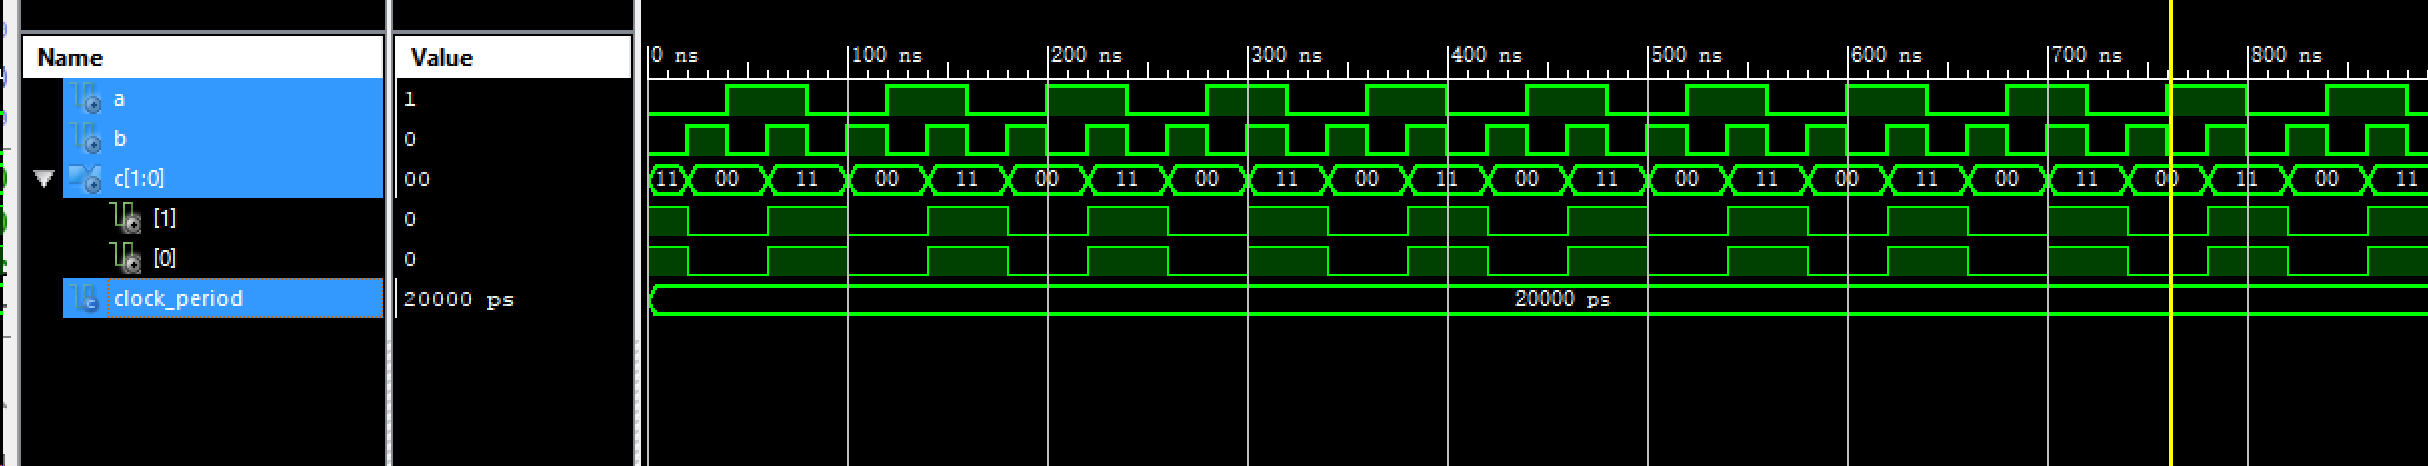
\includegraphics[width=1\linewidth]{homework4-1}
\caption{Behavioral Simulation (1)}
\label{fig:homework4-1}
\end{figure}

    \section{RTL Schematic}
    \label{sec:rtlschematic}
    
    For RTL Schematic, the top level schematic is just like figure \ref{fig:homework4-2}.
    And the lower level of the schematic of both RTL and Technology are just like figure \ref{fig:homework4-3}, and figure \ref{fig:homework4-4}.
    
\begin{figure}[h!]
\centering
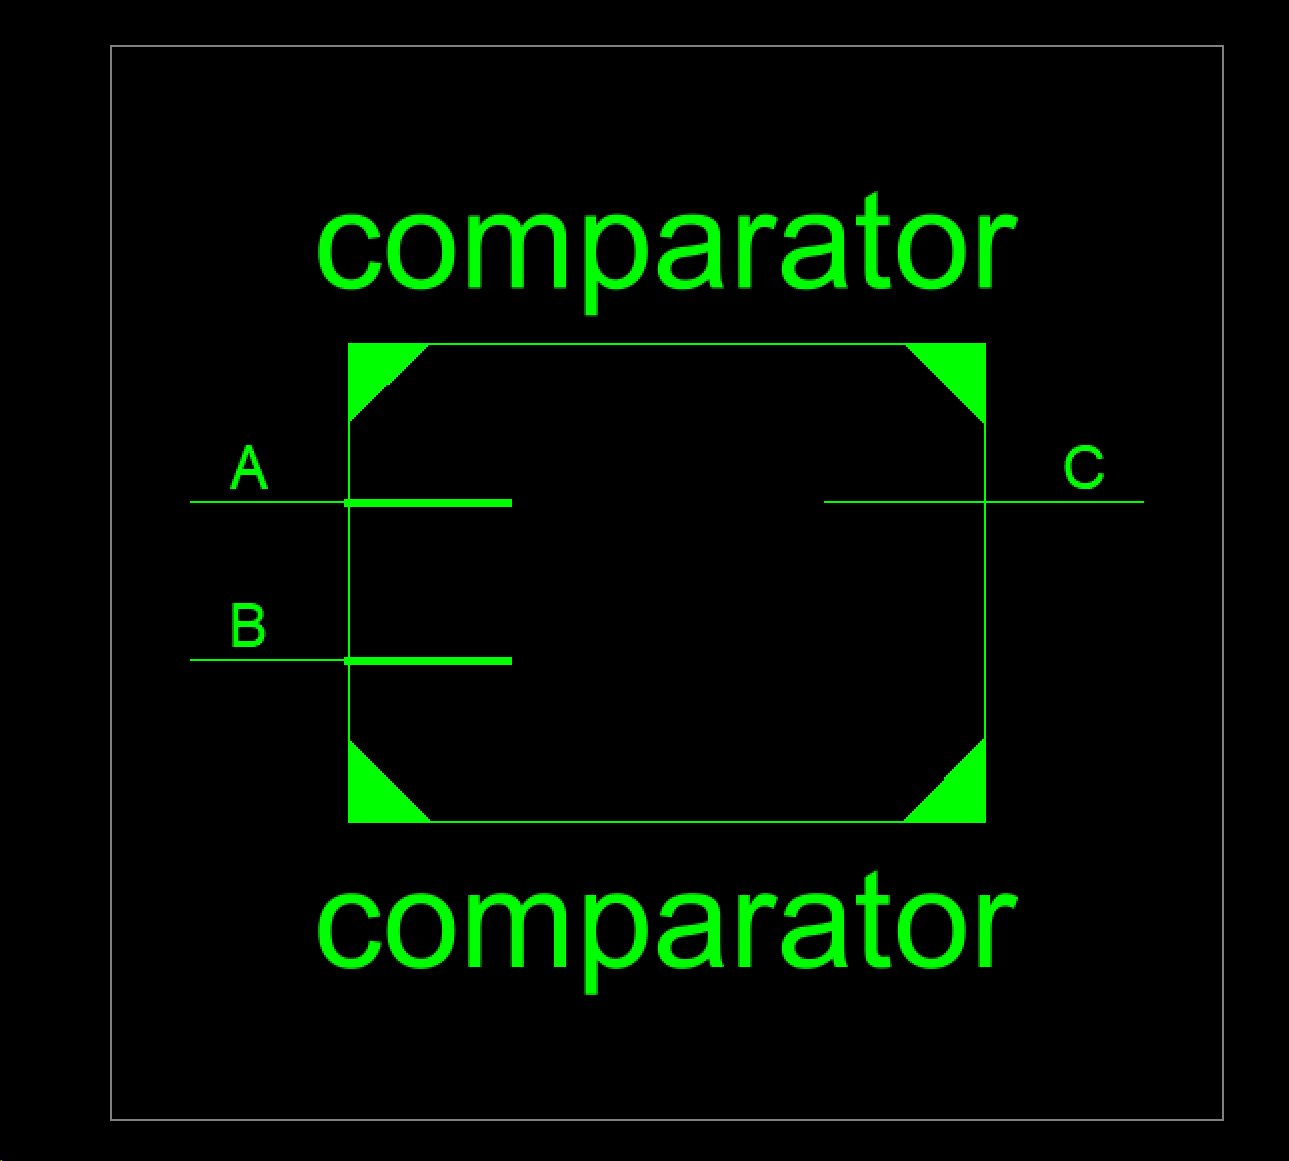
\includegraphics[width=1\linewidth]{homework4-2}
\caption{Top Level of RTL Schematic}
\label{fig:homework4-2}
\end{figure}

\begin{figure}[h!]
\centering
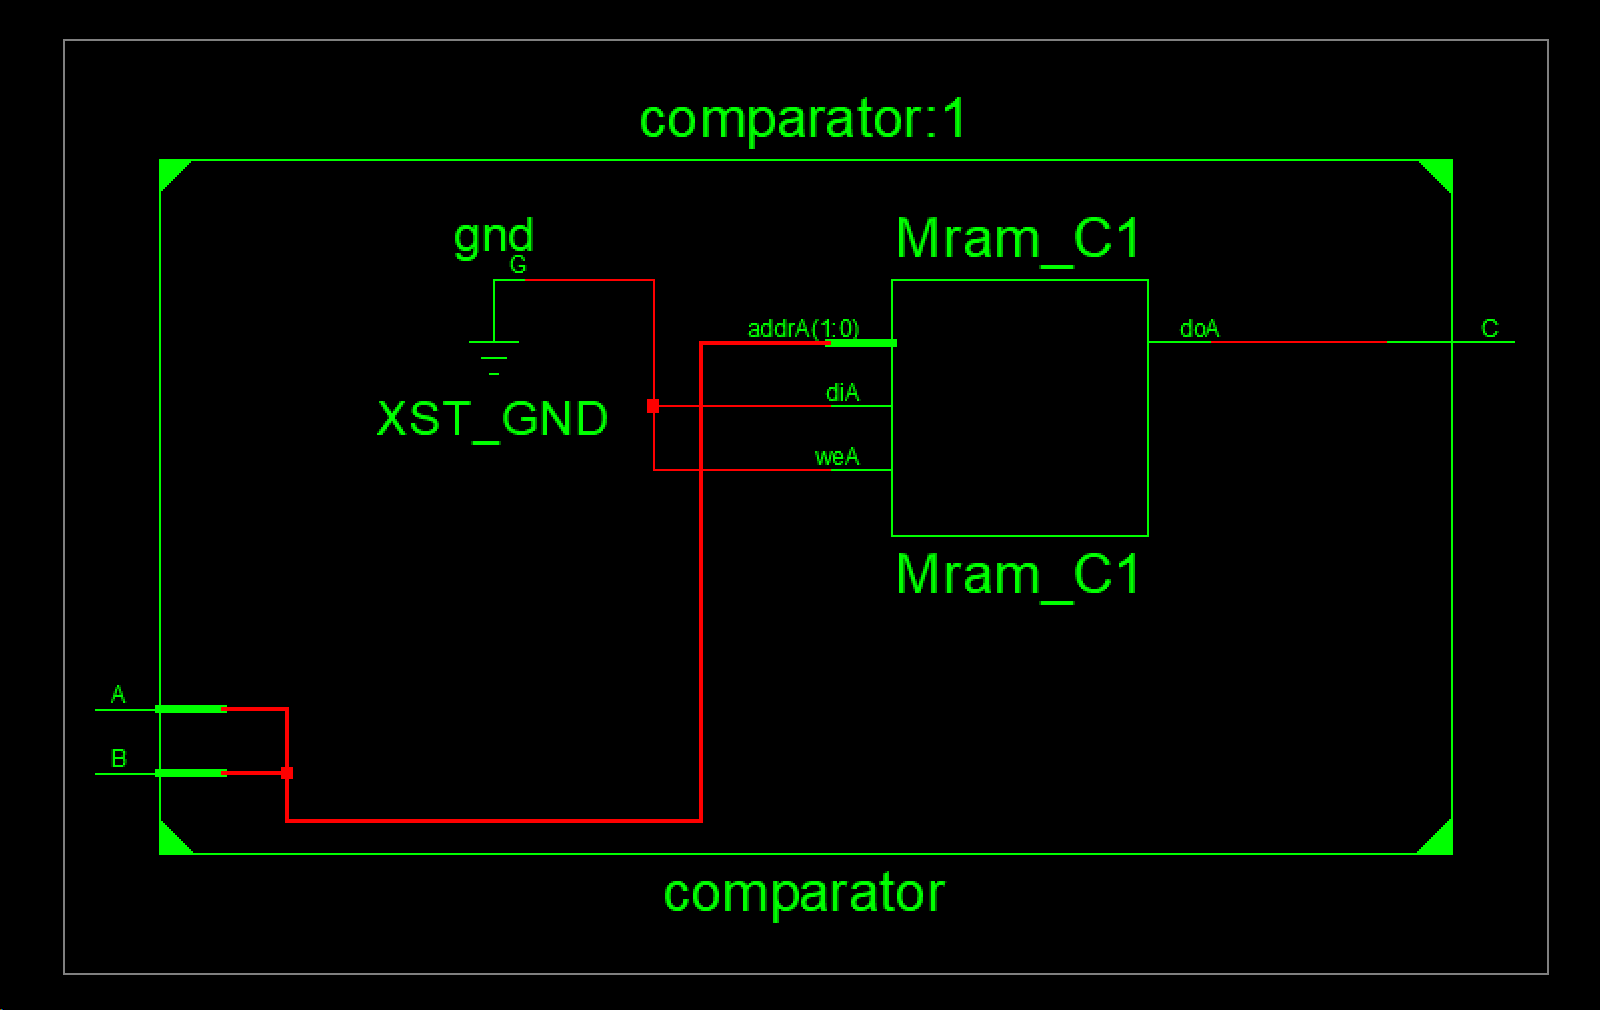
\includegraphics[width=1\linewidth]{homework4-3}
\caption{Lower Level of RTL Schematic}
\label{fig:homework4-3}
\end{figure}

\begin{figure}[h!]
\centering
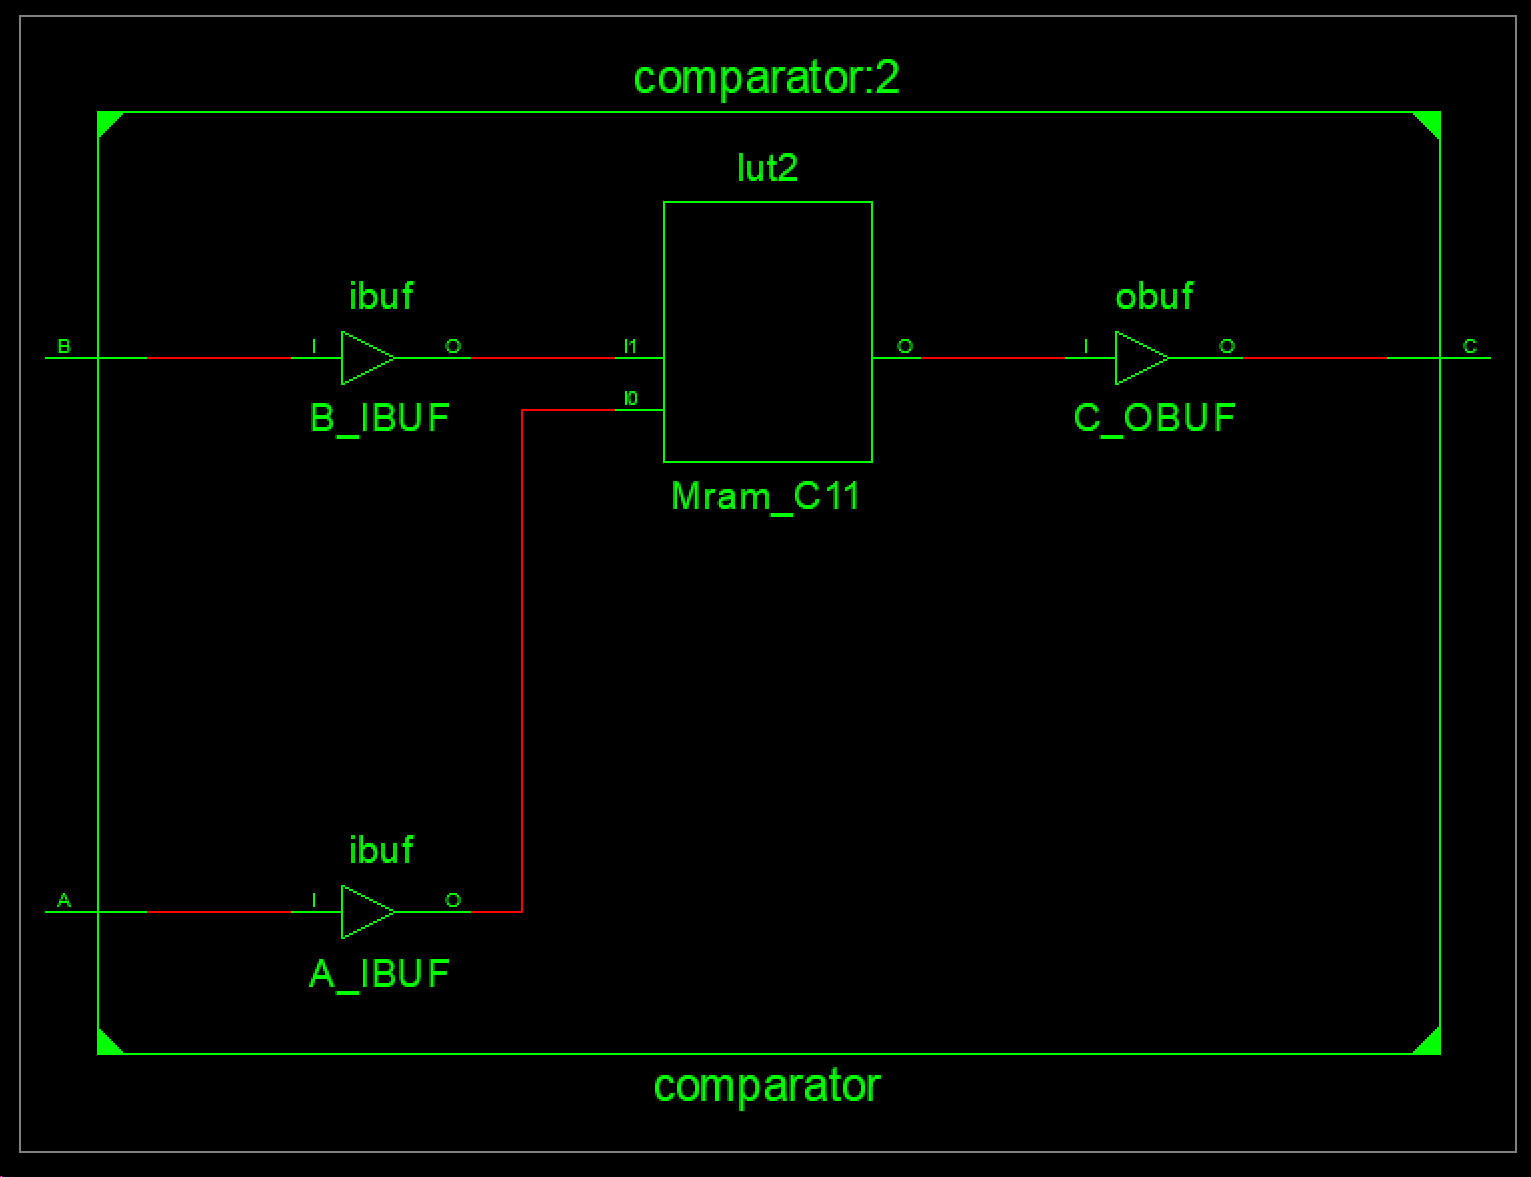
\includegraphics[width=1\linewidth]{homework4-4}
\caption{Lower Level of Technology Schematic}
\label{fig:homework4-4}
\end{figure}


    \section{Post-Route Simulation}
    \label{sec:postroutesimulation}
    
    After placing and routing, the delay of the signal can not be ignore.
    Sometime we might need to reroute or replace when the delay has the bad effect on the signal or
    the circuit.
    
    Back to my comparator, unfortunately, the one using xor can not work because of the delay.
    In the figure \ref{fig:homework4-5}, the delay is almost inacceptable, and its frequency is just 50MHz. When the 100MHz of the input signals' frequency, delay of the signal can not be
    accepted, as the figure \ref{fig:homework4-6}. The signal is also unstable.
    
\begin{figure}[h!]
\centering
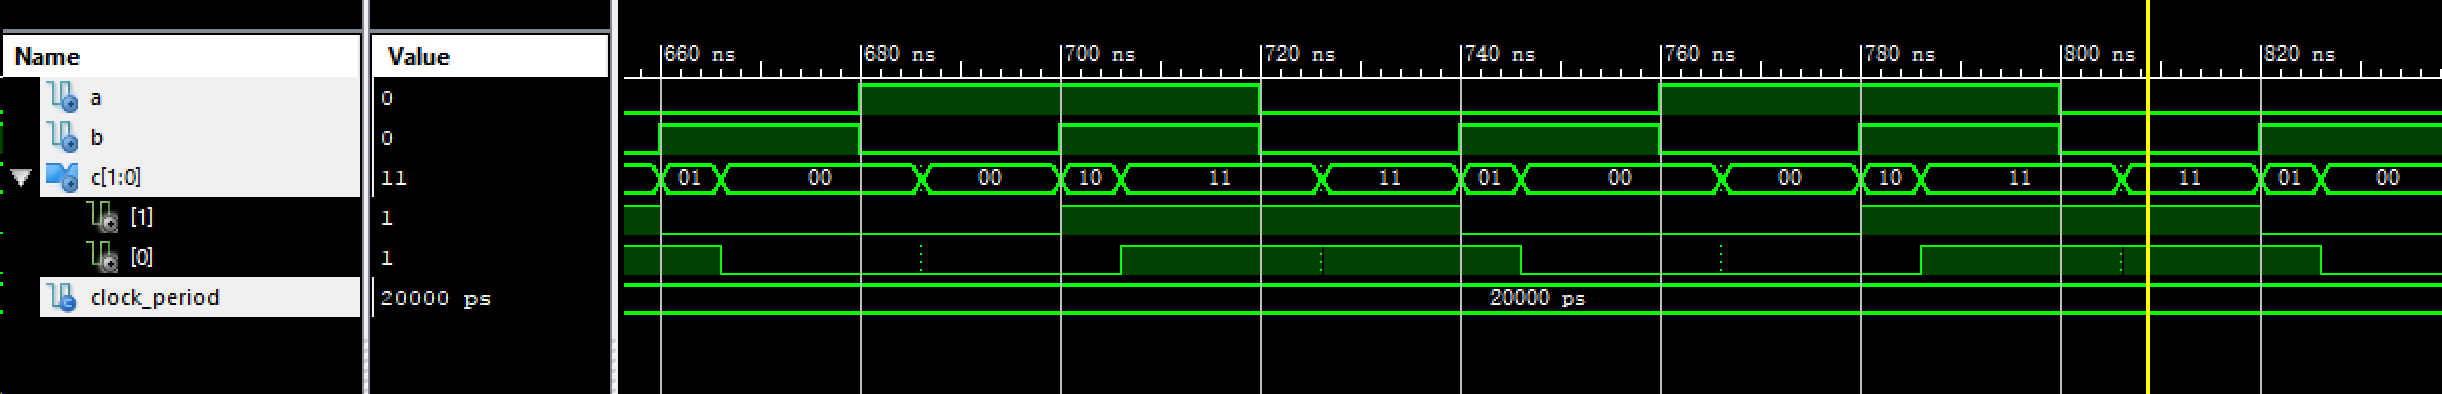
\includegraphics[width=1\linewidth]{homework4-5}
\caption{The Delay of Signals (50MHz)}
\label{fig:homework4-5}
\end{figure}

\begin{figure}[h!]
\centering
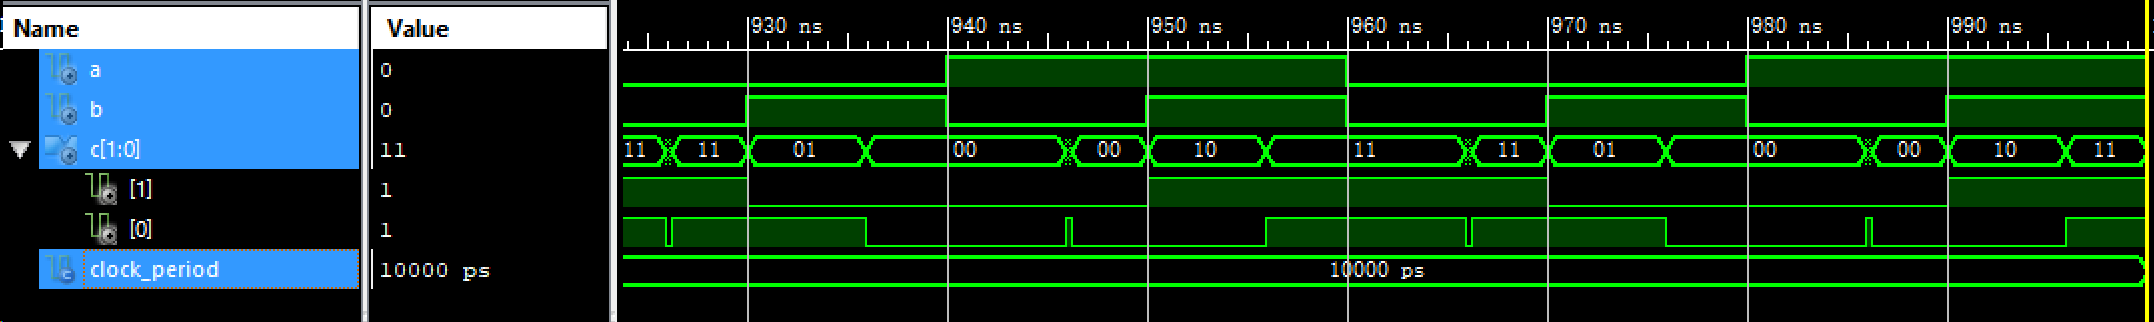
\includegraphics[width=1\linewidth]{homework4-6}
\caption{The Delay of Signals (100MHz)}
\label{fig:homework4-6}
\end{figure}

    For the one with with-select notation, the delay is almost zero, and has any difference with
    the behavioral simulation. 
    
   
\end{document}